%% =====================================================================
%%  2026-11-16-共同研究者向け説明：共同研究者に研究の全体を説明する資料（日本語だけ）．第 2 版
%%  研究者の依頼（2026-11-16）：「共同研究者に研究を説明するようなスライドpdfを，今の原稿に基づいて作ってほしい．わかりやすさ重視．」
%%  第 2 版の依頼（2026-11-16 午後）：実験設定と提案と比べる相手が直観的に分かる石井・岡田型の図を足す．前半は解析の道具と素朴な
%%  やり方の結果でよい．後半の提案の節で，どのコーパス・モダリティでなぜ良くなるか，提案が効いたか，なぜ既存の方法では足りないかを
%%  詳しく説明する．
%%  元にした原稿：DAI/paper/ja/ の日本語の下書き（コミット 5f82b88 以降．6.5・6.7・7.5 節などに 11-16 の追記あり）と，照合を通した
%%  結果の文（docs/結果/計算の後の解析_提案が効くコーパスの型_2026-11-16.md 第 3 版，計算の後の解析_感情ごとの当たり方_2026-11-16.md
%%  第 8 版，実験23_結果の文の下書き_2026-11-16.md 第 3 版）．
%%  図：fig_overview_study_ja・fig_fusion_map_ja・fig_corpus_types_ja は第 2 版で作った図（台本 DAI/paper/scripts/make_figs_overview.py，
%%  make_fig_corpus_types.py）．ほかは原稿の図（英語）．
%%  数値：原稿の説明なので，数値は照合を通した原稿の文と結果の文から写した（slides/CLAUDE.md の決まり 2 の例外．各ページの出所に書いた）．
%% =====================================================================
\input{preamble}
\input{merda}

\newcommand{\T}[2]{#1}
\newcommand{\msg}[1]{\par\vspace{0.25em}{\centering\large #1\par}}
\newcommand{\fnote}[1]{\par\vfill{\tiny\color{mMuted}#1\par}}
\newcommand{\notreal}{\par{\tiny\color{mMuted}模式図．実験の値ではない}\par}
\newcommand{\figsrc}[1]{\par\vspace{-0.2em}\hfill{\tiny\color{mMuted}#1}\par}
\newcommand{\pt}{点}
\newcommand{\qbox}[2]{\par\noindent\fcolorbox{#1}{#1!8}{\parbox{\dimexpr\linewidth-2\fboxsep-2\fboxrule}{\raggedright\footnotesize #2}}\par\vspace{0.3em}}
\definecolor{qOne}{HTML}{8E2457}\definecolor{qTwo}{HTML}{3B2F8F}\definecolor{qThree}{HTML}{8A5A00}\definecolor{pOne}{HTML}{882255}\definecolor{pTwo}{HTML}{8C510A}

\title{新しいコーパスに数本のラベルしか無いときの\\マルチモーダル感情認識}
\subtitle{素朴な疑似ラベルはどの分類器で効くか，答えのまとめ方をどう変えるとどのコーパスで効くか}
\author{杉浦 伸一}
\institute{北陸先端科学技術大学院大学}
\date{2026年11月16日　共同研究者への説明（論文の日本語の下書きに基づく．第 2 版）}

\begin{document}
\maketitle

%% ===================================================================== 要約
\begin{frame}{この研究で分かったこと（1 枚で）}
\scriptsize
\qbox{pOne}{\textbf{前半：素朴なやり方（3 つの分類器の確率を同じ重みで掛けた疑似ラベルで学び直す）はどの分類器で効くか．}\\
→ 声の分類器は，感情ごとに 5・10・25 本のラベルしか無い 12 条件すべてで，同じラベルだけで学び直した分類器より \textbf{1.4〜4.1 点}高かった（点推定）．顔・言葉・AVT では一部のコーパスだけだった．上がったのは\textbf{疑似ラベルが学び直す分類器より当たるとき}だけで，声は多くのコーパスで最も強いモダリティではなく，言葉の分類器の判断を顔の特徴より\textbf{よくまねできた}．}
\qbox{pTwo}{\textbf{後半：答えのまとめ方をどう変えると，どのコーパスで効くか．}\\
→ 各分類器の強さを数本のラベルで，感情ごとの得意・不得意をほかのコーパスで測ってまとめる方法（提案）は，どの条件でも積を区間で下回らず，\textbf{1 つのモダリティだけが飛び抜けて強い AFEW で +2.1〜+3.5 点}高かった．AFEW では数本のラベルで測った強さが最も強い顔の分類器を見抜いた．既存のまとめ方は，同じ重みは AFEW で，数本のラベルで重みを合わせる方法は IEMOCAP・MOSEI で提案より低かった（点推定）．}
\fnote{UAR：感情ごとの正解率の平均（4 感情ででたらめに答えると 25）．点：UAR の差の単位．出所：原稿の要旨，1 節，5〜8 節，結果の文（提案が効くコーパスの型，実験 23）．}
\end{frame}

\begin{frame}{研究の全体（1）：設定}
\centering
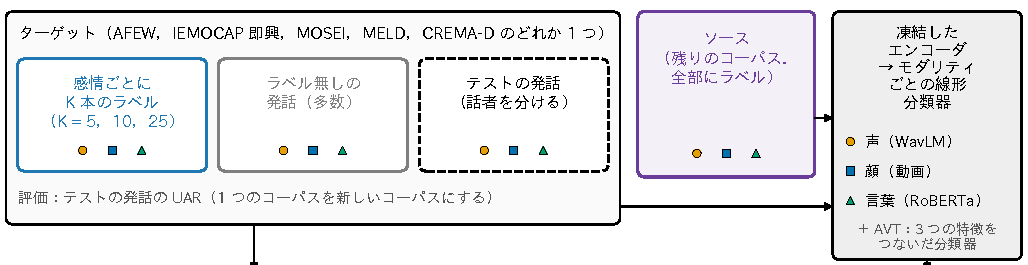
\includegraphics[width=\linewidth,height=0.62\textheight,keepaspectratio]{figures/fig_overview_study_setting_ja.pdf}
\par\vspace{0.4em}\footnotesize\raggedright
新しいコーパス（ターゲット）には感情ごとに K 本のラベルと，ラベル無しの発話がある．ほかのコーパス（ソース）は全部にラベルがある．声・顔・言葉の凍結した特徴の上に線形分類器を置き，話者を分けたテストの発話の UAR で評価する．
\notreal
\end{frame}

\begin{frame}{研究の全体（2）：前半と後半}
\centering
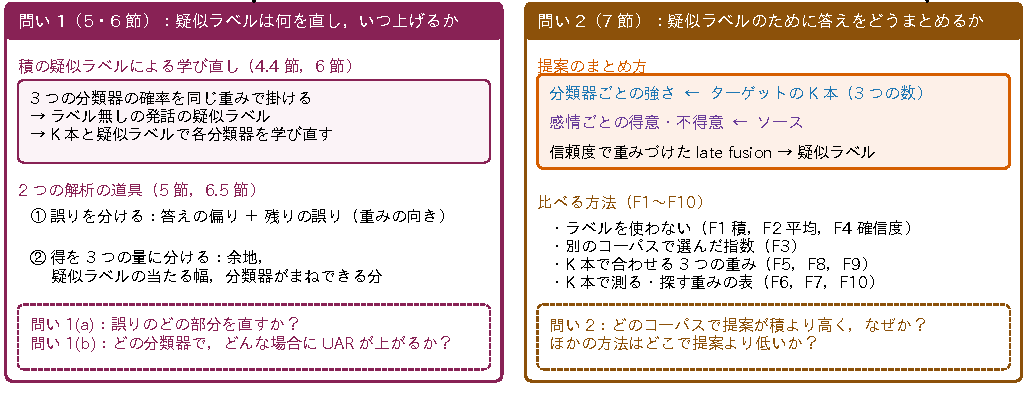
\includegraphics[width=\linewidth,height=0.80\textheight,keepaspectratio]{figures/fig_overview_study_parts_ja.pdf}
\notreal
\end{frame}

%% ===================================================================== 設定
\section{設定}

\begin{frame}{背景と問い}
\begin{columns}[T]
\begin{column}{0.5\textwidth}
\footnotesize
\textbf{背景}
\begin{itemize}\setlength\itemsep{2pt}
\item 感情のコーパスは，録音の環境，演技か自然な表出か，ラベルの付け方が違う．1 つのコーパスで学んだ分類器は，ほかのコーパスで成績が落ちることが報告されている
\item ラベルは複数の評定者が付けるので高い．ラベルの無い録音は集めやすい
\item これまで：ほかのモダリティの分類器の予測（\key{疑似ラベル}）をラベル無しの録画に付け，それを目標に声の分類器を学ぶ方法（Albanie ほか 2018，Zhang ほか 2021）
\end{itemize}
\end{column}
\begin{column}{0.47\textwidth}
\footnotesize
\textbf{この研究の設定}\\
新しいコーパス（\key{ターゲット}）には感情ごとに \key{K 本}（5，10，25）だけラベルがある．ほかのコーパス（\key{ソース}）は全部にラベルがある．ターゲットの残りの発話はラベル無し．
\vspace{0.5em}

\textbf{問い}
\begin{enumerate}\setlength\itemsep{2pt}
\item 疑似ラベルで学び直すと，どの分類器の UAR が上がり，なぜか（前半）
\item 声・顔・言葉の答えをどうまとめて疑似ラベルにすれば，どのコーパスで良くなり，なぜか（後半）
\end{enumerate}
\end{column}
\end{columns}
\fnote{出所：原稿 1 節，2 節．K 本は感情ごとの本数（K = 5 なら 4 感情 × 5 = 20 本）．}
\end{frame}

\begin{frame}{データ：コーパスを 1 つずつ新しいコーパスにした}
\footnotesize
\resizebox{\linewidth}{!}{\begin{tabular}{@{}lllrr@{}}
\toprule
コーパス & 中身 & ラベルの付け方 & 話者 & 発話 \\
\midrule
AFEW & 映画の場面 & 人が場面を見て付けた表情 & 282 & 795 \\
IEMOCAP（即興） & 実験室の 2 人の即興の対話 & 評定者の最多票 & 10 & 2,943 \\
MOSEI & YouTube の独話 & 6 感情の強さから本研究の規則で & 2,626\textsuperscript{*} & 18,919 \\
MELD & ドラマの多人数の会話 & 評定者の多数決 & 283 & 11,343 \\
CREMA-D（後半だけ） & 決まった文の演技（声と顔） & 演じた感情 & 91 & 4,900 \\
\bottomrule
\end{tabular}}
\vspace{0.6em}
\begin{itemize}\setlength\itemsep{2pt}
\item 感情は 4 つ（Neutral，Happy，Sad，Angry）にそろえた．
\item \textbf{話者を分けた}：同じ話者の発話が学習側と評価側の両方に入らない（\textsuperscript{*}MOSEI は話者の注釈が無いので，チャンネルか動画で分けた）．
\item \textbf{LOCO 評価}：4 コーパスの 1 つを新しいコーパス（ターゲット），残る 3 つをソースにする．
\end{itemize}
\fnote{出所：原稿 3 節の表 1（4 感情に絞った後の数．単一ソース設定と全ソース設定の声の集合の値で，LOCO 評価で使った数は原稿の表 4）．IEMOCAP は台本の部を除いた．}
\end{frame}

\begin{frame}{分類器と，この資料で使う言葉}
\scriptsize
\begin{columns}[T]
\begin{column}{0.4\textwidth}
\textbf{特徴}（このコーパスで微調整していない）
\begin{itemize}\setlength\itemsep{1pt}
\item 声：WavLM-large の最終層（1,024 次元）
\item 顔：表情のデータで学んだ ResNet-50（512 次元）
\item 言葉：RoBERTa（768 次元）．AFEW は Whisper の書き起こしから
\item AVT：3 つをつないだ特徴
\end{itemize}
各特徴の上に\textbf{線形分類器}を置く．新しい構造の提案ではなく，情報源ごとに分類器の何が変わるかを測るための設定．
\end{column}
\begin{column}{0.57\textwidth}
\begin{tabular}{@{}p{0.3\linewidth}p{0.66\linewidth}@{}}
\toprule
\key{K 本の基準の分類器} & ソースの分類器の重みの平均を出発点にして，K 本のラベルだけで学び直した分類器．比べる基準 \\
\key{積} & 声・顔・言葉の 3 つの分類器の確率を同じ重みで掛けた答え．素朴な疑似ラベル \\
\key{学び直し} & K 本のラベルと，ラベル無しの発話の疑似ラベルで分類器を学び直すこと \\
\key{gain} & 学び直した分類器 − K 本の基準の分類器の UAR の差 \\
\key{区間} & 95\% 区間（多重比較の補正なし）．「上がった」は区間の下端 > 0 \\
\bottomrule
\end{tabular}
\end{column}
\end{columns}
\fnote{出所：原稿 3.3 節，3.4 節，5.1 節．}
\end{frame}

%% ===================================================================== 前半
\section{前半：解析の道具と，素朴なやり方}

\begin{frame}{道具 1：誤りを「答えの偏り」と「残りの誤り」に分ける}
\begin{columns}[T]
\begin{column}{0.55\textwidth}
\centering
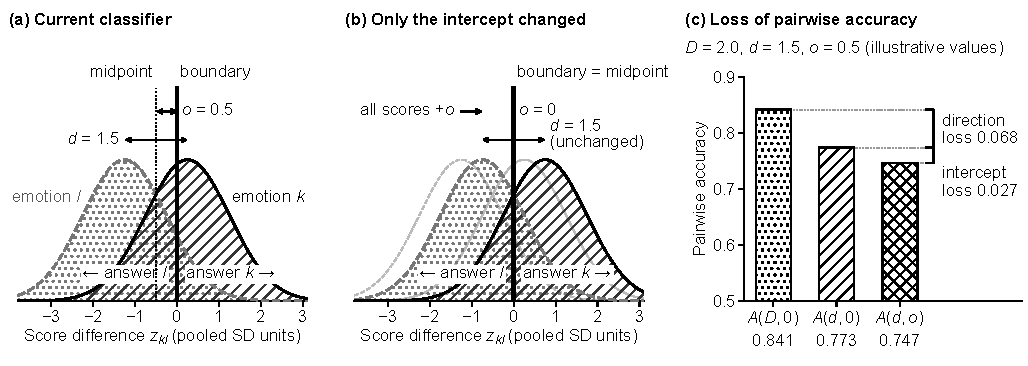
\includegraphics[width=\linewidth,height=0.48\textheight,keepaspectratio]{figures/fig2_decomposition.pdf}
\figsrc{原稿の図 2（数値は説明のための例）}
\scriptsize\raggedright
\textbf{答えの偏り}：境目が真ん中からずれて，答えが一方の感情に偏る部分．境目をずらすだけで直る．\\
\textbf{残りの誤り}：偏りを直しても残る部分（重みの向きのずれ）．
\end{column}
\begin{column}{0.43\textwidth}
\scriptsize
\textbf{4 つの情報源が直した誤り}
\begin{itemize}\setlength\itemsep{2pt}
\item \textbf{ほかのコーパスを混ぜる}：得はラベルが少ないときだけ（K = 1 で +6.9〜+13.4 点，全部のラベルでは $-$2.1〜$-$4.8 点）
\item \textbf{K 本のラベル}：主に偏りを直した．偏りはラベル無しで特徴の平均を引くだけでほぼ直った（声，K = 5．ソースだけの分類器に対して，ソースと K 本をまとめて学ぶと +5.26 点，平均を引くだけで +4.69 点．その後 K 本で切片を直しても +0.38 [$-$0.12, +0.88]）
\item \textbf{同じモダリティのラベル無しの発話}（8 手法）：残りの誤りを減らした条件は 210 のうち 7
\item \textbf{ほかのモダリティの疑似ラベル}：残りの誤りを減らした条件は 81 のうち 38
\end{itemize}
\end{column}
\end{columns}
\fnote{出所：原稿 6.1〜6.4 節（6.1〜6.3 節は 1 つのソースだけを使う設定，6.4 節は全ソースを使う設定）．}
\end{frame}

\begin{frame}{素朴なやり方の結果：声の分類器は 12 条件すべてで基準より高かった}
\begin{columns}[T]
\begin{column}{0.6\textwidth}
\centering
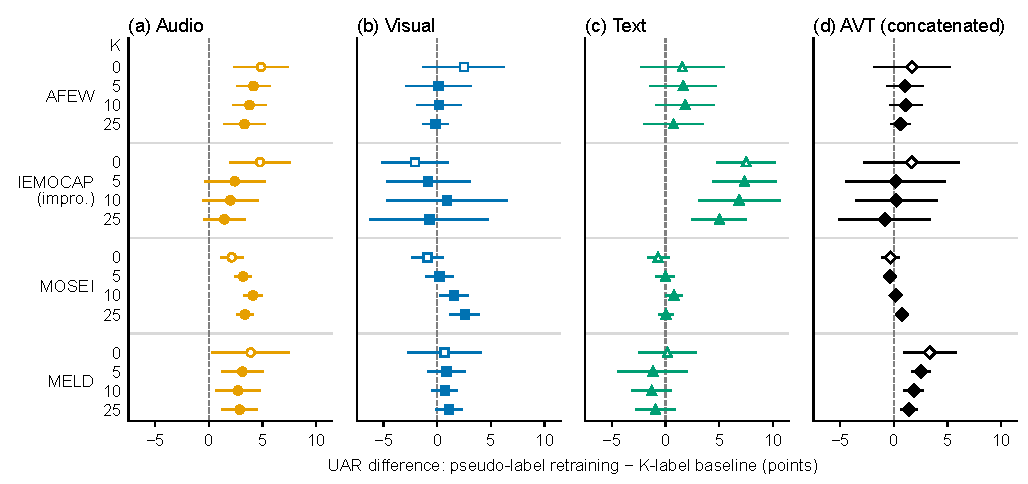
\includegraphics[width=\linewidth,height=0.80\textheight,keepaspectratio]{figures/fig3_q1_retraining.pdf}
\figsrc{原稿の図 3（gain：積の疑似ラベルで学び直し − K 本の基準）}
\end{column}
\begin{column}{0.38\textwidth}
\scriptsize
\textbf{声}：4 コーパス × K = 5，10，25 の 12 条件すべてで点推定が正（+1.4〜+4.1 点）．区間の下端 > 0 は 12 のうち 9（IEMOCAP の 3 つの K は区間が 0 を含む）．ラベルを使わない K = 0 でも 4 コーパスすべてで正（+2.1〜+4.9）．\\[3pt]
\textbf{言葉}：区間の下端 > 0 は IEMOCAP だけ（+5.0〜+7.3）．MELD は $-$1.3〜$-$0.9．\\[3pt]
\textbf{顔}：区間の下端 > 0 は MOSEI の K = 10・25 だけ．\\[3pt]
\textbf{AVT}：区間の下端 > 0 は MELD の 3 つの K と MOSEI の K = 25．\\[3pt]
損失の形を替えても，声の差は $-$0.79〜+0.87 点しか変わらなかった．
\end{column}
\end{columns}
\fnote{出所：原稿 5.3〜5.5 節．}
\end{frame}

\begin{frame}{道具 2：学び直しの得を 3 つの量に分ける}
\begin{columns}[T]
\begin{column}{0.58\textwidth}
\centering
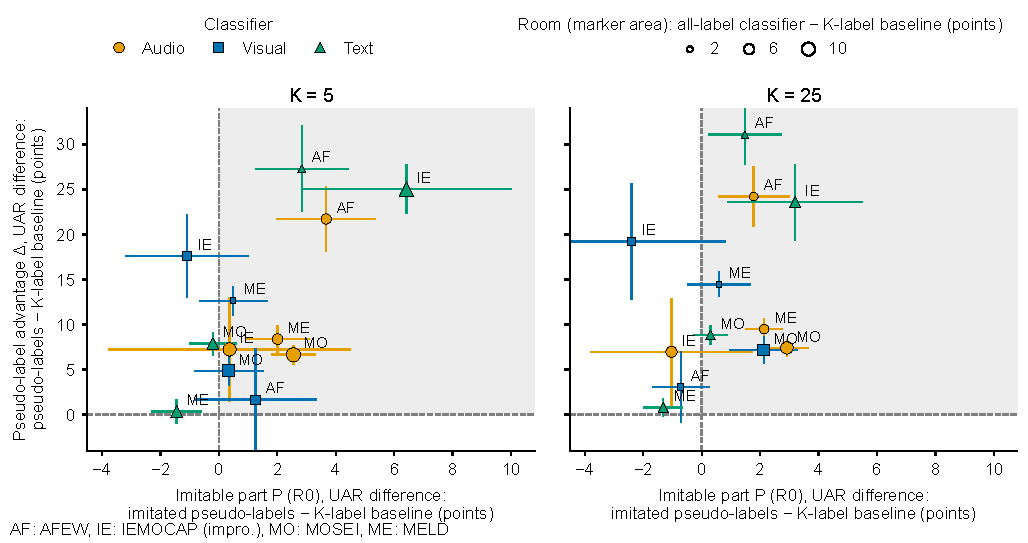
\includegraphics[width=\linewidth,height=0.78\textheight,keepaspectratio]{figures/fig6_conditions.pdf}
\figsrc{原稿の図 6（声・顔・言葉の分類器）}
\end{column}
\begin{column}{0.4\textwidth}
\scriptsize
\textbf{3 つの量}（どれも K 本の基準の分類器との差）
\begin{enumerate}\setlength\itemsep{1pt}
\item \textbf{余地}：全ラベルで学べば上がる分
\item \textbf{当たる幅 Δ}：疑似ラベルの判定のほうがどれだけ当たるか
\item \textbf{再現できる分 P}：その判定を学び直す分類器の特徴でどれだけまねできるか
\end{enumerate}
gain の区間が 0 を上回った声・顔・言葉の分類器では，3 つの量の点推定が正だった（例外は K = 25 の声の AFEW の P で，そろえた読み出しで $-$1.7）．
\end{column}
\end{columns}
\fnote{出所：原稿 6.5 節．}
\end{frame}

\begin{frame}{なぜ声か（1）：疑似ラベルのほうが当たるときだけ上がった}
\begin{columns}[T]
\begin{column}{0.6\textwidth}
\centering
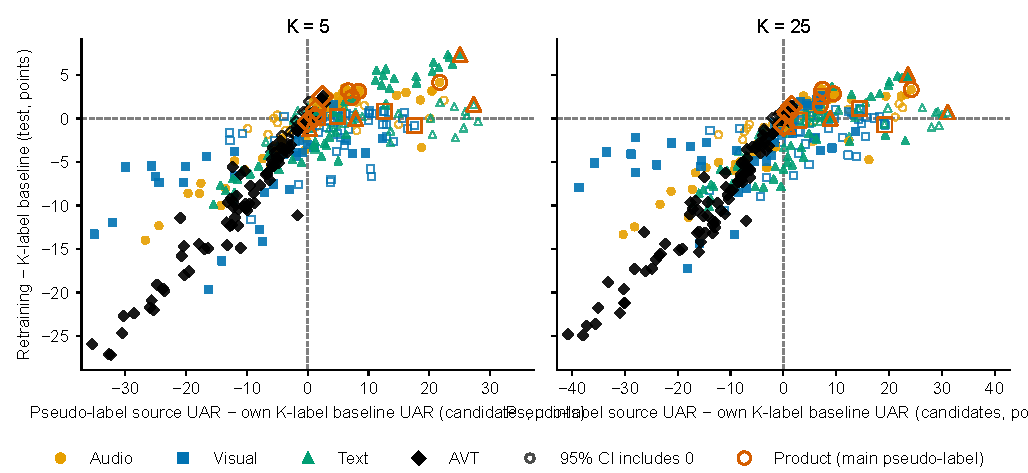
\includegraphics[width=\linewidth,height=0.62\textheight,keepaspectratio]{figures/fig10_teacher_margin.pdf}
\figsrc{原稿の図 10．横軸：当たる幅．縦軸：gain}
\end{column}
\begin{column}{0.38\textwidth}
\scriptsize
疑似ラベルの作り方を替えた学び直しを並べた（K = 5，25 で 360 組ずつ．自分の予測だけの疑似ラベルは除く）．
\begin{itemize}\setlength\itemsep{2pt}
\item 当たる幅と gain の順位相関：0.80，0.83
\item 疑似ラベルのほうが当たらない組には，gain の区間の下端 > 0 は無かった
\item \textbf{最も強いモダリティ}は，ほかの 2 つのモダリティの疑似ラベルで学び直すと 8 例すべてで点推定が負で，区間の上端 < 0 は 5 例（AFEW の顔 \bad{$-$4.4}，\bad{$-$3.2}，MELD の言葉 \bad{$-$3.7}，\bad{$-$4.2}，MOSEI の顔の K = 5 \bad{$-$3.3}．K = 5，25）
\item 声が最も強いのは IEMOCAP だけで，IEMOCAP では声の gain の区間が 0 を含んだ
\end{itemize}
\end{column}
\end{columns}
\fnote{出所：原稿 6.7 節，8.4 節，5.3 節．計算の後に組んだ記述で，順位相関と数えは検定ではない．}
\end{frame}

\begin{frame}{なぜ声か（2）：声は言葉の分類器の判断をまねできる}
\scriptsize
\textbf{声の特徴は，言葉の分類器の判断を顔の特徴よりよく再現した}（K = 5．感情と話者で説明できる一致を除いた D の差：IEMOCAP +17.3，MOSEI +10.2，MELD +13.9 点）．
\vspace{0.2em}

\textbf{言葉を聞き取れなくしても残るか}（実験 23．予言は計算の前に固定）．
音声を\key{逆再生}すると，Whisper の書き起こしの一致率が偶然の水準を超えた分は 0.005〜0.012（元の音声 0.79〜0.80）になった．
\begin{center}
\begin{tabular}{@{}lccc@{}}
\toprule
 & IEMOCAP & MOSEI & MELD \\
\midrule
言葉の判断を再現する D（元の声 → 逆再生） & 19.3 → 10.5 & 10.5 → 3.1 & 17.7 → 10.5 \\
減った分 & 8.8 [3.0, 14.7] & 7.5 [6.3, 8.6] & 7.2 [4.7, 9.8] \\
逆再生した声 − 顔（言葉の判断の D） & 8.5 [3.8, 13.1] & 2.7 [1.3, 4.1] & 6.7 [3.8, 9.6] \\
\bottomrule
\end{tabular}
\end{center}
顔の判断の再現の減りより点数でも割合でも多く減ったのは MOSEI だけ（6.5 [1.1, 11.8]）．
\takeaway{声が言葉の判断をまねできる分を，聞き取れる言葉だけには帰せない．}
\fnote{出所：原稿 6.5 節，8.2 節，9 節，実験 23 の結果の文 第 3 版．IEMOCAP は検出の力が足りず，MELD は区間が 0 を含んだ．IEMOCAP の 3 語以上の発話だけの版は逆再生した声 − 顔が 4.8 [$-$0.2, 9.8]．300 Hz の低域通過は言葉を消し切れず（0.15〜0.39），結果は 6.5 節にあるが言葉を消した操作としては扱わない．}
\end{frame}

\begin{frame}{なぜ声か（3）：AVT は最初から強く，疑似ラベルから学ぶものが少ない}
\scriptsize
\textbf{AVT の当たる幅 Δ}（K = 5．積の疑似ラベル − AVT の K 本の基準．候補の上）
\begin{center}
\begin{tabular}{@{}lcccc@{}}
\toprule
 & AFEW & IEMOCAP & MELD & MOSEI \\
\midrule
当たる幅 Δ & +1.33 [$-$1.3, +4.0] & +1.22 [$-$1.1, +3.6] & \textbf{+2.46 [+1.6, +3.4]} & +0.02 [$-$0.4, +0.5] \\
\bottomrule
\end{tabular}
\end{center}
\begin{itemize}\setlength\itemsep{3pt}
\item 積の疑似ラベルの判定は，AVT の特徴の上の線形の判定で全部の候補について表せた（AVT は積を原理的にまねできる）．
\item AVT の K 本の基準の分類器は，声・顔・言葉の K 本の基準の分類器より強かった（2 つの K とも，12 組のうち点推定で 11 組，区間で 10 組）．
\item 当たる幅の区間の下端 > 0 は MELD だけで，AVT の gain が 3 つの K とも区間の下端 > 0 だったのも MELD だけだった．
\end{itemize}
\takeaway{声は疑似ラベルより弱く（当たる幅が大きい），その判断をまねもできる．AVT は疑似ラベルとほぼ同じ答えを最初から出せる．}
\fnote{出所：実験 22 の結果の文 第 4 版（原稿 6.5 節の表 9 は小数 1 桁），原稿 8.2 節．}
\end{frame}

\begin{frame}{感情ごとに見ると：当たる幅の大きい感情ほど差が大きく，Neutral は点推定で負が多い}
\scriptsize
\begin{itemize}\setlength\itemsep{3pt}
\item \textbf{1 つの組の中で}：疑似ラベルの当たる幅が相対的に大きい感情ほど，その感情の再現率の差も大きかった（4 感情の平均を引いた順位相関 0.56〜0.58．最大の感情が一致した組は 360 のうち 172〜180，偶然の見込み 78〜85）．積で学び直した AVT は，48 の（コーパス，感情，K）すべてで再現率の差の符号が当たる幅の符号と同じだった．
\item \textbf{声の分類器}：Angry の再現率の差は 12 条件すべてで点推定が正（区間の下端 > 0 は 8）．Neutral は IEMOCAP，MELD，MOSEI の 8 条件で点推定が負（区間の上端 < 0 は MELD の 2）．AFEW の Neutral は区間の下端 > 0．
\item \textbf{Neutral が下がる理由の一部}：主な損失は感情ごとの疑似ラベルの重みの合計をそろえる．この操作だけを外す除去実験（評価の前に決めた比べ）と比べると，そろえる操作は Neutral の再現率を 48 条件すべてで点推定で下げ（区間の上端 < 0 は 26），UAR は声の 12 条件で $-$0.78〜+0.12 点しか変えなかった（区間はどれも 0 を含む）．
\item 学び直すと，テストの上の答えの 4 感情の割合は 0.21〜0.29 に寄った（K 本の基準の分類器は 0.14〜0.38）．テストの正解の Neutral の割合は AFEW 0.26 から MELD 0.57 まで．
\end{itemize}
\fnote{出所：原稿 5.3 節，5.5 節，6.7 節，8.2 節．結果の文（感情ごとの当たり方）第 8 版．計算の後に組んだ記述．}
\end{frame}

\begin{frame}{前半のまとめ：なぜ声の分類器だけが安定して上がったか}
\footnotesize
\begin{enumerate}\setlength\itemsep{6pt}
\item \textbf{疑似ラベルのほうが当たる}：声は多くのコーパスで最も強いモダリティではない．疑似ラベルが学び直す分類器より当たらない組では，UAR は上がらず，最も強いモダリティでは下がった．
\item \textbf{疑似ラベルの判断をまねできる}：声の特徴は言葉の分類器の判断を顔の特徴よりよく再現した．その分は，言葉を聞き取れなくしても一部残った．
\item \textbf{疑似ラベルと同じ答えを最初から出せる分類器（AVT）は，学ぶものが少ない}．
\end{enumerate}
\vspace{0.6em}
\takeaway{素朴な積でも，疑似ラベルの当たり方は学び直す分類器より良いことが多い．では，疑似ラベルそのものをもっと当たるようにできるか ─ これが後半の問い．}
\fnote{出所：原稿 6.5 節，6.7 節，8.2 節．}
\end{frame}

%% ===================================================================== 後半
\section{後半：疑似ラベルのための答えのまとめ方}

\begin{frame}{提案の動機：強さはコーパスで入れ替わり，感情ごとの形は似ていた}
\begin{columns}[T]
\begin{column}{0.6\textwidth}
\centering
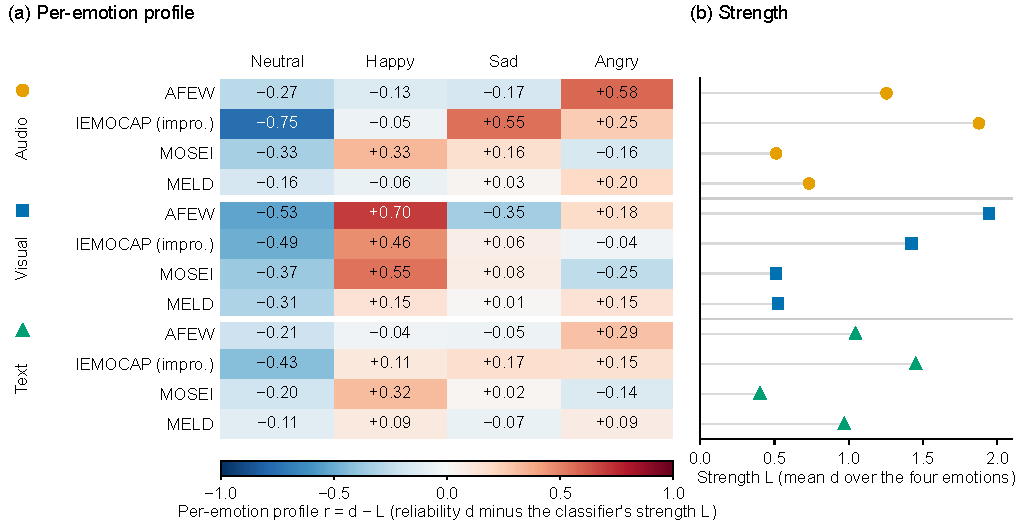
\includegraphics[width=\linewidth,height=0.80\textheight,keepaspectratio]{figures/fig7_strength_profile.pdf}
\figsrc{原稿の図 7（設定を決めるための計算の値．評価の回の値ではない）}
\end{column}
\begin{column}{0.38\textwidth}
\scriptsize
\begin{itemize}\setlength\itemsep{3pt}
\item \textbf{強さ（水準）}：3 つの分類器のどれが強いかはコーパスで入れ替わった．ほかのコーパスで測った強さで最も強い分類器が合った割合は 0〜0.47（K 本で測ると 0.43〜1.00）
\item \textbf{得意・不得意の形（相性）}：強さを除いた感情ごとの形は，コーパスをまたいで似ていた（相関 0.46〜0.78）
\item 道具 1 から，K 本のラベルは主に偏りを直す．そこで K 本からは分類器ごとに \textbf{1 つの数（強さ）}だけを測る
\end{itemize}
\end{column}
\end{columns}
\fnote{出所：原稿 7.1 節．}
\end{frame}

\begin{frame}{提案：強さは K 本で，感情ごとの形はソースで測ってまとめる}
\centering
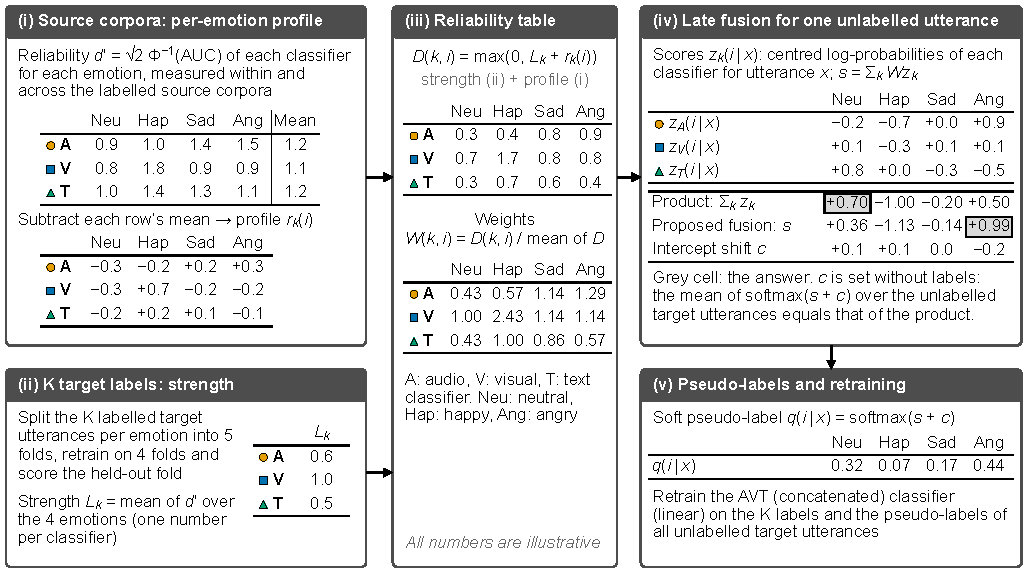
\includegraphics[width=0.84\linewidth,height=0.56\textheight,keepaspectratio]{figures/fig8_method.pdf}
\par\footnotesize\raggedright
(i) ソースで分類器 × 感情の信頼度を測り，行の平均を引いて「形」にする．(ii) ターゲットの K 本で分類器ごとの「強さ」を 1 つ測る．(iii) 強さ + 形で重みの表を作る．(iv) ラベル無しの発話ごとに，3 つの分類器の点数を重みづけて足す（late fusion）．(v) その答えを疑似ラベルにして，AVT の分類器を学び直す．
\figsrc{原稿の図 8（表の数値は説明のための例）}
\end{frame}

\begin{frame}{何と比べたか：重みをどこから決めるか}
\begin{columns}[T]
\begin{column}{0.62\textwidth}
\centering
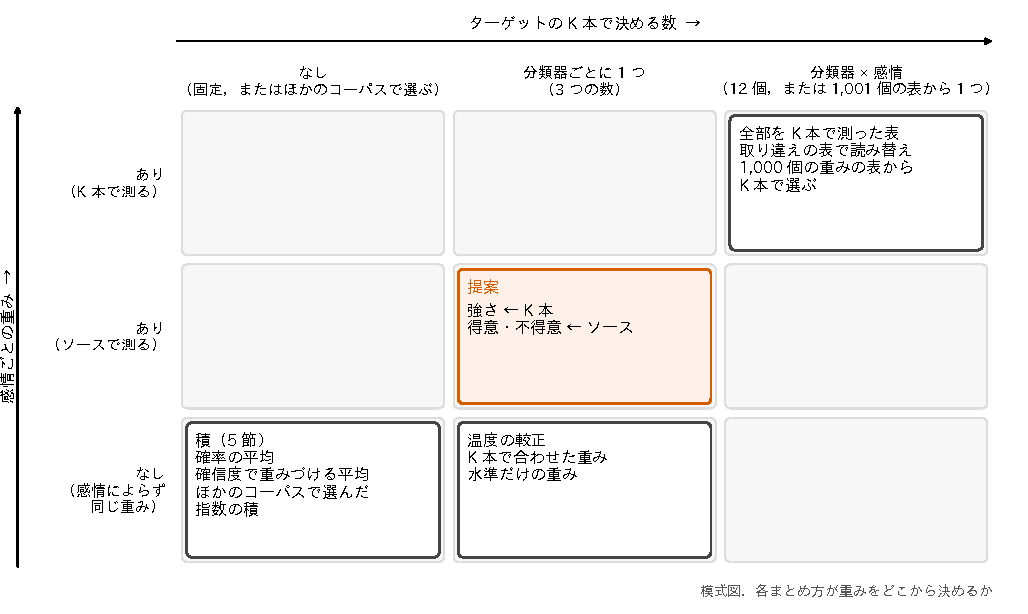
\includegraphics[width=\linewidth,height=0.80\textheight,keepaspectratio]{figures/fig_fusion_map_ja.pdf}
\end{column}
\begin{column}{0.36\textwidth}
\scriptsize
同じ 3 つの分類器と同じ K 本を使い，\textbf{答えのまとめ方だけ}を替えた．
\begin{itemize}\setlength\itemsep{2pt}
\item \textbf{同じ重み}：積（素朴なやり方），確率の平均，確信度で重みづける平均
\item \textbf{ほかのコーパスで選んだ重み}：別のコーパスで選んだ指数の積
\item \textbf{K 本で重みを合わせる}：分類器ごとの温度の較正，K 本で合わせたモダリティごとの重み
\item \textbf{K 本で表を選ぶ・測る}：乱数の重みの表 1,000 個と等しい重みの表の 1,001 個から K 本の UAR で選ぶ，12 個の信頼度を全部 K 本で測る
\end{itemize}
提案は「K 本で決めるのは 3 つの強さだけ，感情ごとの形はソース」の位置にある．
\end{column}
\end{columns}
\fnote{出所：原稿 7.3 節の表 10．評価のターゲットの K 本・候補・テストは前半と同じ．50 反復（5 分割 × K 本の引き方 10）．}
\end{frame}

\begin{frame}{結果：提案は積を 12 条件のうち 11 で点推定で上回った}
\begin{columns}[T]
\begin{column}{0.6\textwidth}
\centering
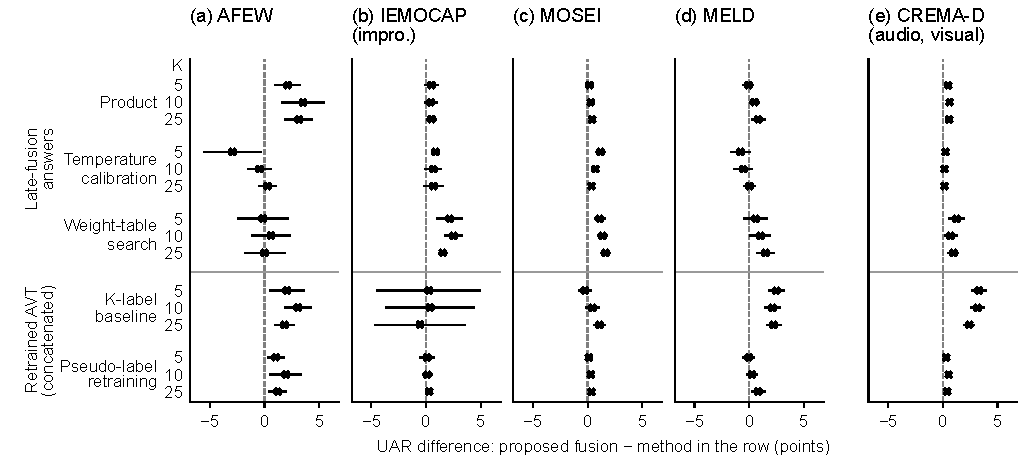
\includegraphics[width=\linewidth,height=0.80\textheight,keepaspectratio]{figures/fig9_fusion_vs_others.pdf}
\figsrc{原稿の図 9}
\end{column}
\begin{column}{0.38\textwidth}
\scriptsize
まとめた答え（疑似ラベルにする前）の提案 − 積
\begin{itemize}\setlength\itemsep{2pt}
\item 4 コーパス × K = 5，10，25 の 12 条件のうち 11 で点推定が正，7 条件で区間の下端 > 0
\item \textbf{AFEW：+2.13，+3.51，+3.14 点}
\item IEMOCAP，MOSEI，MELD：$-$0.09〜+0.83 点
\item CREMA-D（声と顔だけ）：+0.47，+0.63，+0.57（区間の下端 > 0）
\end{itemize}
疑似ラベルで学び直した AVT どうし（提案 − 積）：AFEW で +1.01，+1.95，+1.21（区間の下端 > 0），ほかの 9 条件で $-$0.05〜+0.82．
\end{column}
\end{columns}
\fnote{出所：原稿 7.4 節．結果の文（提案が効くコーパスの型）第 3 版の要点 19．}
\end{frame}

\begin{frame}{どのコーパスで効いたか（1）：分類器の強さの並び方}
\centering
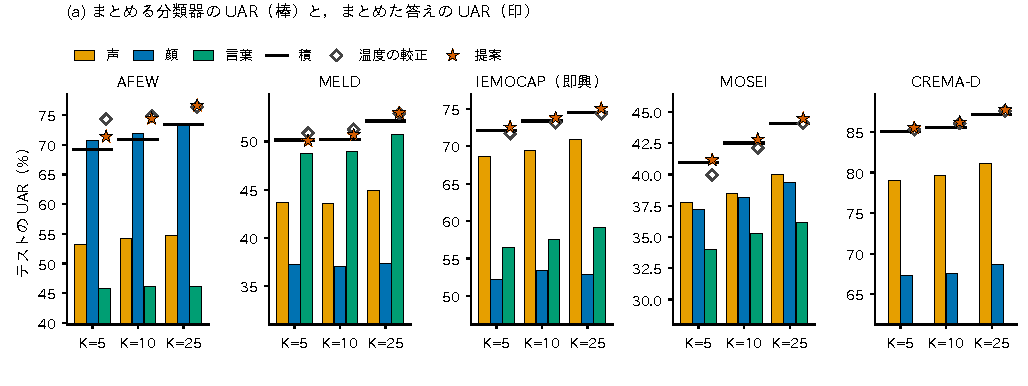
\includegraphics[width=\linewidth,height=0.58\textheight,keepaspectratio]{figures/fig_corpus_types_a_ja.pdf}
\par\vspace{0.2em}\scriptsize\raggedright
\textbf{AFEW} は顔が声より 17.5〜18.6 点強く，同じ重みの積は顔の分類器 1 つにも届かなかった（積 − 顔：$-$1.47，$-$1.05，+0.21）．ここで提案（★）が積（横線）を大きく上回った．\textbf{MELD} は言葉が強いが，積は言葉の分類器より 1.25〜1.45 点高い．\textbf{IEMOCAP，MOSEI，CREMA-D} では，積が最も強い単独の分類器より 3.2〜6.1 点高く，提案と積の差は小さい．
\fnote{出所：結果の文（提案が効くコーパスの型）第 3 版の要点 19．棒は積を作る 2 段目の分類器のテストの UAR．CREMA-D は分類器が 2 つ（声と顔）の別の回の値．}
\end{frame}

\begin{frame}{どのコーパスで効いたか（2）：提案の得は AFEW で最も大きかった}
\centering
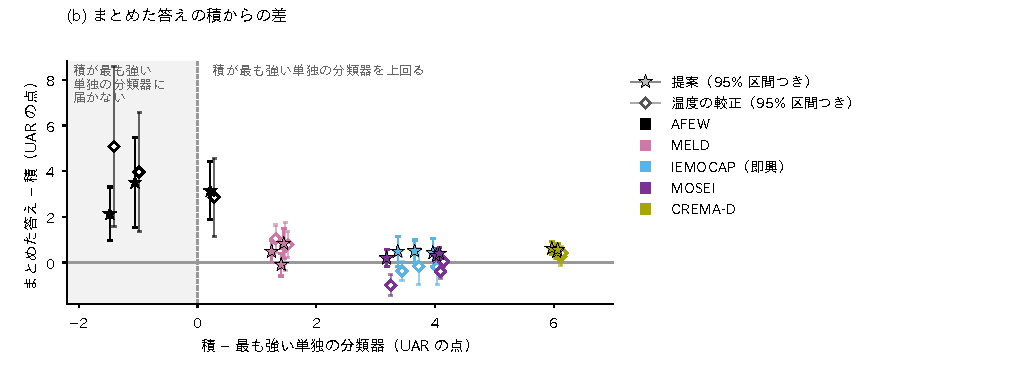
\includegraphics[width=\linewidth,height=0.58\textheight,keepaspectratio]{figures/fig_corpus_types_b_ja.pdf}
\par\vspace{0.1em}\scriptsize\raggedright
提案 − 積は，AFEW で 3 つの K とも 5 コーパスの中で最も大きかった（+2.13〜+3.51）．積が最も強い単独の分類器を 1.25〜6.07 点上回るほかの 4 コーパスでは $-$0.09〜+0.83 で，この 4 つの並びは K で入れ替わった．温度の較正（◇）は AFEW の K = 5・10 で提案より大きく積を上回り（K = 25 では提案のほうが大きい），MOSEI の K = 5・10 では区間でも積を下回った．
\fnote{出所：結果の文（提案が効くコーパスの型）第 3 版の要点 19・20．計算の後に並べ直した記述．2 つの軸はどちらも積の UAR を含むので，逆向きの関係が式の上で入る．}
\end{frame}

\begin{frame}{なぜ効いたか：AFEW では強さを K 本で見抜いた}
\scriptsize
\begin{itemize}\setlength\itemsep{4pt}
\item \textbf{提案の重み}（4 感情の平均）：AFEW では顔が最大（顔，声，言葉の順に K = 5 で 1.17，0.93，0.90，K = 10 で 1.32，0.87，0.81）．IEMOCAP では声が最大（K = 5 で 1.19）．
\item \textbf{K 本で測った強さは最も強い分類器を当てた}：評価の 50 反復で，K 本で測った強さが最も強い分類器を選んだ割合は AFEW 0.94〜1.00，IEMOCAP 0.86〜1.00，MELD 0.70〜0.88．\textbf{ほかのコーパスで測った強さ}はいつも同じ分類器を選び，AFEW では声，IEMOCAP と MELD では顔で，3 つとも外れた．MOSEI は 1 位と 2 位の差が小さく，K 本でも 0.30〜0.38（でたらめに選ぶのと同じ水準）．
\item \textbf{部品を外すと}：AFEW では，分類器どうしの強さの違いを外す段で +1.74〜+3.20 点下がった（6 つとも区間の下端 > 0）．MOSEI では，感情ごとの形（相性）を外す段で +0.48〜+0.73 点下がった．相性を外した版との差は，CREMA-D を含む 15 条件すべてで点推定が正（+0.10〜+0.73）．
\item \textbf{得は「向き」の側に出た}：差を「答えの偏りを直す分」と「それ以外（向きの分）」に分けると，偏りの分は 12 条件とも区間が 0 を含み（$-$0.42〜+0.17），向きの分は AFEW で +2.55，+3.87，+3.35．
\end{itemize}
\takeaway{1 つの分類器が特に強い AFEW では，その強さを数本のラベルで測れたことが効いた．MOSEI と CREMA-D では，ソースで測った感情ごとの形が少し上乗せした．}
\fnote{出所：原稿 7.4〜7.6 節，8.3 節．}
\end{frame}

\begin{frame}{既存のまとめ方は，どこで提案より低かったか}
\scriptsize
推定時の答えの「提案 − 相手」（4 コーパス × K = 5，10，25．* は区間の下端 > 0，† は上端 < 0，‡ は 0 に近い端が引き直しの乱数に依りうる）
\vspace{0.2em}
\begin{center}
\resizebox{\linewidth}{!}{\begin{tabular}{@{}lllll@{}}
\toprule
相手の型 & AFEW & IEMOCAP & MOSEI & MELD \\
\midrule
同じ重み（確率の平均） & +2.14\textsuperscript{*}，+3.38\textsuperscript{*}，+3.73\textsuperscript{*} & $-$0.46，$-$0.46，$-$0.49 & +0.15，+0.26，+0.52\textsuperscript{*} & $-$0.22，+0.30，+0.65 \\
ほかのコーパスで選んだ指数の積 & +2.13\textsuperscript{*}，+3.51\textsuperscript{*}，+3.14\textsuperscript{*} & +2.52\textsuperscript{*}，+2.36\textsuperscript{*}，+2.72\textsuperscript{*} & +0.45\textsuperscript{‡}，+0.49\textsuperscript{*}，+0.57\textsuperscript{*} & +2.10\textsuperscript{*}，+2.42\textsuperscript{*}，+2.94\textsuperscript{*} \\
温度の較正（K 本） & \bad{$-$2.94\textsuperscript{†}}，$-$0.45，+0.27 & +0.87\textsuperscript{*}，+0.64，+0.67 & +1.18\textsuperscript{*}，+0.69\textsuperscript{*}，+0.36\textsuperscript{*} & $-$0.80，$-$0.56，+0.04 \\
K 本で合わせた重み & $-$3.54，$-$1.57，$-$1.50 & +2.30\textsuperscript{*}，+1.38\textsuperscript{*}，+0.90\textsuperscript{*} & +2.30\textsuperscript{*}，+1.61\textsuperscript{*}，+0.90\textsuperscript{*} & +0.57，$-$0.15，$-$0.08 \\
1,000 個の表から K 本で選ぶ & $-$0.14，+0.59，+0.03 & +2.15\textsuperscript{*}，+2.50\textsuperscript{*}，+1.54\textsuperscript{*} & +1.10\textsuperscript{*}，+1.34\textsuperscript{*}，+1.66\textsuperscript{*} & +0.59，+1.01\textsuperscript{*}，+1.48\textsuperscript{*} \\
\bottomrule
\end{tabular}}
\end{center}
\begin{itemize}\setlength\itemsep{2pt}
\item \textbf{同じ重み}は，1 つが飛び抜けて強い AFEW で提案より低かった．
\item \textbf{ほかのコーパスで選んだ重み}は，強さの順が入れ替わる IEMOCAP と MELD で低かった（AFEW では指数が (1,1,1) で積と同じ）．
\item \textbf{K 本で重みを合わせる・表を選ぶ方法}は，AFEW では提案との差の区間がほとんど 0 を含み（区間で相手が高いのは温度の較正の K = 5 だけ），IEMOCAP と MOSEI では点推定で 18 条件すべて提案より低かった（区間で 16．0 を含むのは温度の較正の IEMOCAP の K = 10・25）．
\end{itemize}
\fnote{出所：結果の文（提案が効くコーパスの型）第 3 版の要点 20（effects.csv．照合済み）．原稿 7.4 節の表 11．}
\end{frame}

\begin{frame}{温度の較正との比べ：重みの差のつけ方が違った}
\scriptsize
\begin{columns}[T]
\begin{column}{0.5\textwidth}
\textbf{差の符号の数}（推定時の答え，提案 − 温度の較正）
\begin{itemize}\setlength\itemsep{2pt}
\item 12 条件のうち点推定で正 8，負 4（AFEW の K = 5・10，MELD の K = 5・10）
\item 区間で数えると，提案が高い 4（IEMOCAP の K = 5，MOSEI の 3 つの K），低い 1（AFEW の K = 5：$-$2.94 [$-$5.60, $-$0.29]）
\item 学び直した AVT どうしでは，IEMOCAP と MOSEI の 6 条件すべてで提案が高く（区間の下端 > 0），AFEW の K = 5・10 と MELD の K = 10 で低かった（区間の上端 < 0）
\end{itemize}
\textbf{温度の較正 − 積}：AFEW +5.07，+3.96，+2.87，MELD +0.71，+1.04，+0.79，IEMOCAP $-$0.38，$-$0.21，$-$0.16，\bad{MOSEI $-$0.99，$-$0.40}（区間の上端 < 0），+0.04．提案は 15 条件のどれでも積を区間で下回らなかった．
\end{column}
\begin{column}{0.47\textwidth}
\textbf{重みの比}（K = 5，10，25）
\begin{center}
\begin{tabular}{@{}lcc@{}}
\toprule
 & 温度の較正 & 提案 \\
\midrule
AFEW 顔 ÷ 声 & 2.21，1.89，1.44 & 1.27，1.52，1.30 \\
MELD 言葉 ÷ 声 & 1.64，1.57，1.41 & 1.02，1.11，1.25 \\
MOSEI 顔 ÷ 声 & 1.30，1.24，1.27 & 1.00，1.02，1.01 \\
\bottomrule
\end{tabular}
\end{center}
温度の較正は，AFEW・MELD・MOSEI で重みにより大きな差をつけた（IEMOCAP では同じか提案のほうが大きい）．\\[3pt]
提案が K 本で測った強さを等しいほうへ戻す設定（n0 = 20）を仮のターゲットで選んだのは AFEW の K = 5・25 と MELD の K = 5・10．戻さない版との差は AFEW の K = 5 で $-$1.59\textsuperscript{†}，MELD の K = 5 で $-$0.59\textsuperscript{†}．戻さない版は評価の後には採らない．
\end{column}
\end{columns}
\fnote{出所：結果の文（提案が効くコーパスの型）第 3 版の要点 20・21，原稿 7.4 節．計算の後の記述．重みの比の違いは記述で，差の理由とは書かない．}
\end{frame}

%% ===================================================================== 考察
\section{考察と限界}

\begin{frame}{新しいコーパスで手間をどこに回すか（示唆）}
\footnotesize
\begin{enumerate}\setlength\itemsep{5pt}
\item \textbf{ラベル無しのマルチモーダルの録画を集め，疑似ラベルで学び直す．}声の分類器は，ラベル無しの発話と疑似ラベルだけ（K = 0）でも，感情ごとに 5 本と 10 本のラベルで学び直した基準を 4 コーパスすべてで上回った．
\item \textbf{疑似ラベルが学び直す分類器より当たるかを見る．}当たらない組では UAR は上がらず，最も強いモダリティの分類器は下がりうる．
\item \textbf{数本のラベルは，各分類器の強さを測るのに使う．}1 つのモダリティが強いコーパスで効いた．K 本から取り違えの表を推して疑似ラベルを補正する使い方では上がらなかった．
\end{enumerate}
\vspace{0.4em}
\textbf{注意}：疑似ラベルが当たるか（当たる幅）は候補の全ラベルで測った量で，数本のラベルで見積もれるかは調べていない．
\fnote{出所：原稿 8.4 節．}
\end{frame}

\begin{frame}{限界}
\footnotesize
\begin{itemize}\setlength\itemsep{4pt}
\item \textbf{範囲}：4 つの英語のコーパス（後半は CREMA-D を加えた 5 つ）と，声・顔・言葉に 1 組ずつのエンコーダ．
\item \textbf{設定}：凍結した特徴の上の線形分類器．エンコーダを微調整する場合は調べていない．
\item \textbf{同じデータで説明と手法を作った}：手法の形は評価に使ったコーパスの上で作り，提案の案は前半の評価の出力を見た後に立てた．積などとの差は提案に有利な向きに偏りうる．
\item \textbf{計算の後の記述}：コーパスの型，感情ごとの解析，K 本とソースで測った強さの比べは，結果を見た後に組んだ記述で，5 コーパスからの並びである．
\item \textbf{言葉を聞き取りにくくする操作}：逆再生は Whisper で確かめたが，人の聞き手では確かめていない．低域通過は言葉を消し切れなかった．
\item \textbf{区間}：多重比較の補正をしていない．コーパスの数え上げは検定ではない．
\end{itemize}
\fnote{出所：原稿 9 節．}
\end{frame}

%% ===================================================================== まとめ
\section{まとめ}

\begin{frame}{まとめ}
\footnotesize
\begin{itemize}\setlength\itemsep{6pt}
\item \textbf{問題}：新しいコーパスに感情ごとに数本のラベルしか無いとき，ほかのコーパス，ラベル無しの発話，ほかのモダリティをどう使うか．
\item \textbf{前半}：誤りを 2 つに，学び直しの得を 3 つの量に分ける道具を作った．素朴な積の疑似ラベルで学び直すと，声の分類器は 12 条件すべてで +1.4〜+4.1 点（点推定）．上がるのは疑似ラベルのほうが当たり，その判断をまねできるとき．
\item \textbf{後半}：強さを数本のラベルで，感情ごとの形をソースで測ってまとめると，積を 12 条件のうち 11 で点推定で上回り，どの条件でも区間で下回らなかった．1 つのモダリティが飛び抜けて強い AFEW で +2.1〜+3.5 点．
\end{itemize}
\vspace{0.5em}
\takeaway{新しいコーパスでは，ラベル無しのマルチモーダルの録画を集めて疑似ラベルで学び直し，数本のラベルは各分類器の強さを測るのに使う．}
\end{frame}

%% ===================================================================== 補足
\appendix
\section*{補足}

\begin{frame}{補足：用語と原稿の節の対応}
\scriptsize
\begin{tabular}{@{}p{0.24\linewidth}p{0.48\linewidth}p{0.2\linewidth}@{}}
\toprule
用語 & この資料での意味 & 原稿 \\
\midrule
LOCO 評価 & 4 コーパスの 1 つをターゲット，残る 3 つをソースにする & 4.3 節 \\
単一ソース設定 & ソースのコーパス 1 つとターゲットの K 本で学ぶ設定 & 4.3 節，6.1〜6.3 節 \\
全ソース設定 & ターゲット以外の全群のアンカーから K 本で学び直す設定 & 4.3 節，6.4 節 \\
アンカー（出発点） & ソースの分類器の重みと切片の平均 & 5.1 節 \\
積 & 声・顔・言葉の 2 段目の分類器の確率を同じ重みで掛けた答え & 5.1 節 \\
当たる幅・再現できる分 & 学び直しの得を分ける 3 つの量のうちの 2 つ & 6.5 節 \\
水準・相性 & 提案の重みの 2 つの成分（分類器の強さ，感情ごとの形） & 7.2 節 \\
切片の分・向きの分 & 提案 − 積を，切片を合わせ直す手順で分けた 2 つの部分 & 7.6 節 \\
\bottomrule
\end{tabular}
\fnote{この資料は論文の日本語の下書き（DAI/paper/ja/）と，照合を通した結果の文に基づく．}
\end{frame}

\end{document}
